\eject

\section{Solving Linear Systems}

In many contexts where linear systems appear, we are interested in the solutions of that system. Is there a systematic way to solve linear systems? 

\begin{colourframe}[tolGrey]{\bf Big Questions}
	\begin{itemize}
		\item How do we solve systems of linear equations?
		\item How can we use matrices to simplify the process of solving linear systems?
		\item Why don't elementary operations change the solution space of a system?
	\end{itemize}
\end{colourframe}


\subsection*{Elementary Operations}


\begin{example}\label{ex:mixingfood}
	A doctor needs to put a patient on a specific diet consisting of three components, called Food A, Food B, and Food C. The patient must consume exactly 2000 calories per day, 1000mg of sodium per day, and 70g of protein per day. They provide you will the nutritional information of each food and ask you to determine how many servings of each food the patient should consume each day.
	\begin{itemize}
		\item One serving of Food A contains 300 calories, 150mg of sodium, and 10g of protein.
		\item One serving of Food B contains 200 calories, 100mg of sodium, and 20g of protein.
		\item One serving of Food C contains 600 calories, 100mg of sodium, and 20g of protein.
	\end{itemize}
	
	Let $x$ be the number of servings of Food A the patient must consume each day, $y$ the number of servings of Food B the patient must consume each day, and $z$ the number of servings of Food C the patient must consume each day. We know that the patient must consume 2000 calories each day, so we can begin by finding out how many calories they actually consume. Since Food A contains 300 calories per serving and the patient is consuming $x$ servings of Food A, they consume $300x$ calories from eating Food A. Similarly, they consume $200y$ calories from consuming Food B and $600z$ calories from consuming Food C. In total they consume $300x + 200y + 600z$ calories, giving us the following linear equation.
	$$300x + 200y + 600z = 2000$$
	
	Applying similar reasoning to the amount of sodium and protein the patient consumes, we arrive at the following linear system.
	\[
	\arraycolsep=1.4pt
	\begin{array}{rcrcrl}
		300x &+& 200y &+& 600z &= 2000\\
		150x &+& 100y &+& 100z &= 1000\\
		10x &+& 20y &+& 20z&= 70
	\end{array}
	\]
	
	To find the number of servings of each food the patient should consume, we need to solve this system. How can we do that?

\end{example}

As a first step to solving linear systems, we need to understand how we're allowed to manipulate linear systems. The following operations can be performed to any linear system without changing the solution space.

\begin{definition}The \textbf{elementary operations} are:
	\begin{itemize}
		\item Multiply (or divide) an equation by a non-zero constant.
		\item Interchange two equations.
		\item Add a constant multiple of an equation to a different equation.
	\end{itemize}
\end{definition}

The last of these operations is less intuitive than the others. Let's see an example in practice,

\begin{example}
	Consider the linear system $\left\{
			\arraycolsep=1.4pt
			\begin{array}{rcrcrl}
				4x &-& 2y &+& z &= 3\\
						x &&&-& z &= 0
		\end{array}\right.$. How does adding $4$ times the first equation to the second equation change this system?
		
		\begin{center}
			\begin{minipage}{0.2\textwidth}
				\[
				\arraycolsep=1.4pt
				\begin{array}{rcrcrl}
					4x &-& 2y &+& z &= 3\\
					x &&&-& z &= 0
				\end{array}
				\]
			\end{minipage}
			$\xrightarrow{
				\begin{minipage}{0.25\textwidth}
					Add $4$ times the first equation to the second.
				\end{minipage}
				}$
			\begin{minipage}{0.5\textwidth}
				\[
				\arraycolsep=1.4pt
				\begin{array}{rcrcrl}
					4x &-& 2y &+& z &= 3\\
					(1 + 4\times 4)x &- & 2\times 4y&+& (-1 + 4\times 1)z &= 4\times 3
				\end{array}
				\]		
			\end{minipage}
		\end{center}
		
		Note that we still have two equations after applying this operation. We have replaced the second equation $x-z = 0$ in our system by a new equation $17x - 8y +3z = 12$.
\end{example}

It is not immediately obvious that these elementary operations do not change the solution space of a linear system. We consider a concrete example.

\begin{example}
	Suppose we have the linear system, System A
	\[
	\text{System A}
	\]\vspace{-20pt}
	\[
	\arraycolsep=1.4pt
	\begin{array}{rcrl}
		{\color{tolBlue}2x} & {\color{tolBlue}+} & {\color{tolBlue}y} &= {\color{tolBlue}1}\\
		{\color{tolRed}6x} & {\color{tolRed}-} & {\color{tolRed}4y} &= {\color{tolRed}3}
	\end{array}
	\]

	We can perform elementary operations to this system to create new systems of linear equations. System B below is created by multiplying {\color{tolRed}the second equation} in System A by 3. System C is created by interchanging the two equations in System A. System D is created by adding $-2$ times {\color{tolBlue}the first equation} in System A to {\color{tolRed}the second equation.}
	
	\begin{minipage}{0.3\textwidth}
		\[
		\text{System B}
		\]\vspace{-15pt}
		\[
		\arraycolsep=1.4pt
		\begin{array}{rcrl}
			{\color{tolBlue}2x} & {\color{tolBlue}+} & {\color{tolBlue}y} &= {\color{tolBlue}1}\\
			{\color{tolOrange}18x} & {\color{tolOrange}-} & {\color{tolOrange}12y} &= {\color{tolOrange}9}
		\end{array}
		\]
	\end{minipage}
	\begin{minipage}{0.3\textwidth}
		\[
		\text{System C}
		\]\vspace{-15pt}
		\[
		\arraycolsep=1.4pt
		\begin{array}{rcrl}
			{\color{tolRed}6x} & {\color{tolRed}-} & {\color{tolRed}4y} &= {\color{tolRed}3}\\
			{\color{tolBlue}2x} & {\color{tolBlue}+} & {\color{tolBlue}y} &= {\color{tolBlue}1}
		\end{array}
		\]
	\end{minipage}
	\begin{minipage}{0.3\textwidth}
		\[
		\text{System D}
		\]\vspace{-15pt}
		\[
		\arraycolsep=1.4pt
		\begin{array}{rcrl}
			{\color{tolBlue}2x} & {\color{tolBlue}+} & {\color{tolBlue}y} &= {\color{tolBlue}1}\\
			{\color{tolPurple}2x} & {\color{tolPurple}-} & {\color{tolPurple}6y} &= {\color{tolPurple}1}
		\end{array}
		\]
	\end{minipage}

	\vspace{10pt}

	To see the effects of these elementary operations, we can graph each of these systems.

	\begin{center}
		\begin{minipage}{0.24\textwidth}
			\begin{center}
				\begin{tikzpicture}[scale = 0.65]
					\draw[thin, black!20] (-2,-2) grid (2,2);
					\draw[thick, ->] (-2.2, 0) -- (2.2,0) node[right, scale = 0.65]{$x$};
					\draw[thick, ->] (0,-2.2) -- (0,2.2) node[right, scale = 0.65]{$y$};
					
					\foreach \x in {-2,-1,1,2}{
						\draw (\x,0) -- (\x,-0.1) node[below, scale = 0.65]{$\x$};
					}
					\foreach \y in {-2,-1,1,2}{
						\draw (0,\y) -- (-0.1,\y) node[left, scale = 0.65]{$\y$};
					}
					
					\draw[thick, color = tolBlue] (-0.5,2) -- (1.5, -2);
					\draw[thick, color = tolRed] (-0.82,-2) -- (1.84,2);
				
				\end{tikzpicture}\\
				{\scriptsize System A}
			\end{center}
		\end{minipage}
		\begin{minipage}{0.24\textwidth}
			\begin{center}
				\begin{tikzpicture}[scale = 0.65]
					\draw[thin, black!20] (-2,-2) grid (2,2);
					\draw[thick, ->] (-2.2, 0) -- (2.2,0) node[right, scale = 0.65]{$x$};
					\draw[thick, ->] (0,-2.2) -- (0,2.2) node[right, scale = 0.65]{$y$};
					
					\foreach \x in {-2,-1,1,2}{
						\draw (\x,0) -- (\x,-0.1) node[below, scale = 0.65]{$\x$};
					}
					\foreach \y in {-2,-1,1,2}{
						\draw (0,\y) -- (-0.1,\y) node[left, scale = 0.65]{$\y$};
					}
					
					\draw[thick, color = tolBlue] (-0.5,2) -- (1.5, -2);
					\draw[thick, color = tolOrange] (-0.82,-2) -- (1.84,2);
				
				\end{tikzpicture}\\
				{\scriptsize System B}
			\end{center}
		\end{minipage}
		\begin{minipage}{0.24\textwidth}
			\begin{center}			
				\begin{tikzpicture}[scale = 0.65]
					\draw[thin, black!20] (-2,-2) grid (2,2);
					\draw[thick, ->] (-2.2, 0) -- (2.2,0) node[right, scale = 0.65]{$x$};
					\draw[thick, ->] (0,-2.2) -- (0,2.2) node[right, scale = 0.65]{$y$};
					
					\foreach \x in {-2,-1,1,2}{
						\draw (\x,0) -- (\x,-0.1) node[below, scale = 0.65]{$\x$};
					}
					\foreach \y in {-2,-1,1,2}{
						\draw (0,\y) -- (-0.1,\y) node[left, scale = 0.65]{$\y$};
					}
					
					\draw[thick, color = tolBlue] (-0.5,2) -- (1.5, -2);
					\draw[thick, color = tolRed] (-0.82,-2) -- (1.84,2);
				
				\end{tikzpicture}\\
				{\scriptsize System C}
			\end{center}
		\end{minipage}
		\begin{minipage}{0.24\textwidth}
			\begin{center}
				\begin{tikzpicture}[scale = 0.65]
					\draw[thin, black!20] (-2,-2) grid (2,2);
					\draw[thick, ->] (-2.2, 0) -- (2.2,0) node[right, scale = 0.65]{$x$};
					\draw[thick, ->] (0,-2.2) -- (0,2.2) node[right, scale = 0.65]{$y$};
					
					\foreach \x in {-2,-1,1,2}{
						\draw (\x,0) -- (\x,-0.1) node[below, scale = 0.65]{$\x$};
					}
					\foreach \y in {-2,-1,1,2}{
						\draw (0,\y) -- (-0.1,\y) node[left, scale = 0.65]{$\y$};
					}
					
					\draw[thick, color = tolBlue] (-0.5,2) -- (1.5, -2);
					\draw[thick, color = tolPurple] (-2,-0.8333) -- (2,0.5);
				
				\end{tikzpicture}\\
				{\scriptsize System D}
			\end{center}
		\end{minipage}
	\end{center}

	From the graphs, we can see that Systems B and C give the same lines as System A does, and therefore have the same solution space. For System D, we can see that we have changed one of the lines in the system, but that the intersection is still the same. Each of these systems, which we obtained from System A by applying an elementary operation, has the same solution space as System A.

\end{example}

The elementary operations do not change the solution space of a linear system. As such, if we can use them to reduce the system into a simpler form, then these operations can help us solve linear systems. Let us see an example of using these operations to solve a system.

\begin{example}
	Solve the following linear system.
	\[
	\arraycolsep=1.4pt
	\begin{array}{rcrl}
		3x &+& 6y &= 0\\
		2x &-& y &= 5
	\end{array}
	\]
	
	We will use our elementary operations in two ways to solve this system. First, having a coefficient of $1$ in from of $x$ in one of the equations will be easier to work with. The other idea is that adding a multiple of one equation to another can be used to eliminate a variable from an equation. To implement these ideas, we apply the following elementary operations.
	
	\vspace{10pt}
	\begin{minipage}{0.4\textwidth}
		\begin{flushright}
			\vspace{38pt}
		
			Divide the first equation by 3.
			
			\vspace{27pt}
			
			Add $(-2)$ times the first equation to the second.
		\end{flushright}	
	\end{minipage}
	\begin{minipage}{0.35\textwidth}
		\[
		\arraycolsep=1.4pt
		\begin{array}{rcrl}
			3x &+& 6y &= 0\\
			2x &-& y &= 5
		\end{array}
		\]
		
		\vspace{-15pt}
		\begin{center}\rule{30pt}{0.2pt}\end{center}
		
		\vspace{-20pt}
		\[
		\arraycolsep=1.4pt
		\begin{array}{rcrl}
			1x &+& 2y &= 0\\
			2x &-& y &= 5
		\end{array}
		\]
		
		\vspace{-15pt}
		\begin{center}\rule{30pt}{0.2pt}\end{center}
		
		\vspace{-20pt}
		\[
		\arraycolsep=1.4pt
		\begin{array}{rcrl}
			1x &+& 2y &= 0\\
			0x &-& 5y &= 5
		\end{array}
		\]
	
	\end{minipage}
	\begin{minipage}{0.25\textwidth}
		\phantom{a}
	\end{minipage}
	
	\vspace{10pt}
	
	From here, we can see that $y = -1$. We can then substitute $y = -1$ back into our first equation $x + 2y = 0$ to get $x - 2 = 0$, so $x = 2$. Therefore, we get a unique solution of $x = 2$ and $y = -1$. We can verify that it is a solution by substituting back into our original system.

	

\end{example}

This process of substituting $y$ back into the system to find the value of $x$ is refered to as \textbf{back substitution}.

\subsection*{Augment Matrices and Elementary Row Operations}

The previous example was reasonable to do by hand since we had only two equations and two variables. However, if your system is larger, this process can quickly become a lot of writing. To spare ourselves a lot of writing, we have a shorthand for writing out systems of linear equations.

\begin{definition}
	The \textbf{augmented matrix} of a linear system
	\[
	\arraycolsep=1.4pt
	\begin{array}{rcrcccrl}
		a_{11} x_1 &+& a_{12}x_2& +& \dots &+& a_{1n}x_n 	&= b_1\\
		a_{21} x_1 &+& a_{22}x_2& +& \dots &+& a_{2n}x_n 	&= b_2\\
				&	&		&	& \vdots &	&	&	\\
		a_{m1}x_1& +& a_{m2}x_2 &+& \dots &+& a_{mn}x_m &= b_m
	\end{array}
	\]
	is the rectangular array of numbers
	$$\begin{bmatrix}
		a_{11} & a_{12} & \cdots & a_{1n} & b_1\\
		a_{21} & a_{22} & \cdots & a_{2n} & b_2\\
		\vdots &  & & & \vdots\\
		a_{m1} & a_{m2} & \cdots & a_{mn} & b_m
	\end{bmatrix}.$$

\end{definition}

This notation allows us to store all of the information about the system, and eventually manipulate it, with less writing. As a first step in solving linear systems, we will usually consider the system's augmented matrix.

\begin{example}
	The augmented matrix for the system 
		$\left\{
			\arraycolsep=1.4pt
			\begin{array}{rcrcrl}
				4x &-& 2y &+& z &= 3\\
						x &&&-& z &= 0
		\end{array}\right.$
		is $\begin{bmatrix} 4 & -2 & 1 & 3 \\ 1 & 0 & -1 & 0\end{bmatrix}$.
		
		Where did the $0$ in the second row and second column come from? Note that the second column contains the coefficients of $y$ in the linear system. Although $y$ does not appear in the second equation, it remains a variable in the system that we need to represent. We can rewrite the second equation as $x +0y - z = 0$ to make the $0$ coefficient of $y$ apparent.
\end{example}

We will also need to be able to convert from an augmented matrix back into a linear system.

\begin{example}
	Find the linear system corresponding to the augmented matrix 
	$\begin{bmatrix} 1 & 3 & 1\\ 2 & -4 & 3\\4 & 4 & 10\end{bmatrix}.$

	For each row of the augmented matrix, we get an equation. For each column of the augmented matrix, except for the last column, we get a variable. In this case, we have two variables which we will call $x$ and $y$. Then the linear system corresponding to this matrix is:
	\[
	\arraycolsep=1.4pt
	\begin{array}{rcrl}
		x & + & 3y & = 1\\
		2x & - & 4y & = 3\\
		4x & + & 4y & = 10.
	\end{array}
	\]
\end{example}

To solve a linear system, we manipulate the system into a nicer form using elementary operations. Are there corresponding manipulations for the augmented matrix of a system?

\begin{example}
	Consider the following linear system.
	\[
	\arraycolsep=1.4pt
	\begin{array}{rcrl}
		2x & + & 3y  & = 2\\
		x &+&y&=4\\	
		4x & + & y & = 0
	\end{array}
	\]

	To see how elementary operations affect the augmented matrix of a linear system, we will apply the following elementary operations to this system separately, find the augmented matrix of each new system, and then compare with the original augmented matrix.
	
	\begin{center}
		\begin{tabular}{l|c|c}
			Elementary Operation & Linear System & Augmented Matrix\\\hline
			No operation performed. & \begin{minipage}{0.2\textwidth}
				\[
				\arraycolsep=1.4pt
				\begin{array}{rcrl}
					2x & + & 3y  & = 2\\
					x &+&y&=4\\	
					4x & + & y & = 0
				\end{array}
				\]
			\end{minipage}
			& \begin{minipage}{0.2\textwidth} 
				\[\begin{bmatrix} 2 & 3 & 2 \\ 1 & 1 & 4 \\ 4 & 1 & 0\end{bmatrix}\]
			\end{minipage}\\\hline
			Multiply the third equation by 4. & \begin{minipage}{0.2\textwidth}
				\[
				\arraycolsep=1.4pt
				\begin{array}{rcrl}
					2x & + & 3y  & = 2\\
					x &+&y&=4\\	
					\tikzmarkin[hor = style blue]{el} 16x & + & 4y & = 0 \tikzmarkend{el}
				\end{array}
				\]
			\end{minipage}
			& \begin{minipage}{0.2\textwidth} 
				\[
					\begin{bNiceMatrix}
						2 & 3 & 2 \\
						1 & 1 & 4 \\
						\Block[fill = tolBlue!30, rounded-corners]{1-3}{} 16 & 4 & 0
					\end{bNiceMatrix}
				\]
			\end{minipage}\\\hline
			Swap the second and third equations. & \begin{minipage}{0.2\textwidth}
				\[
				\arraycolsep=1.4pt
				\begin{array}{rcrl}
					2x & + & 3y  & = 2\\
					\tikzmarkin[hor = style teal]{al}4x & + & y & = 0\tikzmarkend{al}\\
					\tikzmarkin[hor = style orange]{bl}x &+&y&=4\tikzmarkend{bl}
				\end{array}
				\]
			\end{minipage}
			& \begin{minipage}{0.2\textwidth} 
				\[\begin{bNiceMatrix} 2 & 3 & 2 \\ \Block[fill = tolTeal!40, rounded-corners]{1-3}{}4 & 1 & 0 \\ 
					\Block[fill = tolOrange!40, rounded-corners]{1-3}{}1 & 1 & 4 \end{bNiceMatrix}\]
			\end{minipage}\\\hline
			Add 3 times the second equation to the first. & \begin{minipage}{0.2\textwidth}
				\[
				\arraycolsep=1.4pt
				\begin{array}{rcrl}
					\tikzmarkin[hor = style red]{cl}5x & + &6y  & =14\tikzmarkend{cl}\\
					x &+&y&=4\\	
					4x & + & y & = 0
				\end{array}
				\]
			\end{minipage}
			& \begin{minipage}{0.2\textwidth} 
				\[\begin{bNiceMatrix} \Block[fill = tolRed!40, rounded-corners]{1-3}{}5&  6 & 14 \\ 1 & 1 & 1 \\ 4 & 1 & 0\end{bNiceMatrix}\]
			\end{minipage}
		\end{tabular}
	\end{center}

	Multiplying the third equation in the system by 4 resulted in multiplying each entry in the third row of the augmented matrix by 4. Interchanging the second and third equations in the system resulted in interchanging the second and third rows of the augmented matrix. Lastly, adding 3 times the second equation to the first resulted in adding 3 times the second row to the first. This may be clearer if we rewrite the first row in the last matrix as follows. 
	\[\begin{bmatrix} 2 + 3(1) & 3 + 3(1) & 2 + 3(4) \end{bmatrix}\]
	
	So, when we write ``add 3 times the second row to the first row'', we mean add 3 times the first entry of the second row to the first entry of the first row giving us $2 + 3(1)$,  add 3 times the second entry of the second row to the second entry of the first row giving us $3 + 3(1)$, and  add 3 times the third entry of the second row to the third entry of the first row giving us $2 + 3(4)$. These become the new entries for the first row, in that order.

\end{example}

This example shows that each elementary operation done to the equations of the system also changes the corresponding augmented matrix in a predictable way. From this, we get the \textbf{elementary row operations}.

\begin{definition}
	The elementary row operations are:
	\begin{itemize}
		\item Multiply a row by a non-zero constant.
		\item Interchange two rows.
		\item Add a constant multiple of one row to a different row.
	\end{itemize}
	
	The process of applying elementary row operations to a matrix is called \textbf{row reduction.}

\end{definition}

Let's see how we can use augmented matrices and these elementary row operations to make solving linear systems more straightforward. We return to our nutrition example.

\begin{example}\label{ex:nutrisolve}
	Recall from example \ref{ex:mixingfood} that the doctor's patient must eat $x$ servings of Food A, $y$ servings of Food B, and $z$ servings of Food C each day. By considering their nutritional requirements, we arrived at the following linear system.

	\[
	\arraycolsep=1.4pt
	\begin{array}{rcrcrl}
		300x &+& 200y &+& 600z &= 2000\\
		150x &+& 100y &+& 100z &= 1000\\
		10x &+& 20y &+& 20z&= 70
	\end{array}
	\]

	While we could use elementary equation operations to solve this systen, that will result in a lot of extra writing. So, we will instead work with its augmented matrix. When applying an elementary row operation, we will specify which operation we are applying. You should adopt this practice. It makes keeping track of your work and finding mistakes easier.
	\[
		\setlength{\tabcolsep}{2pt}
		\renewcommand{\arraystretch}{1.5}
		\begin{tabular}{rccc}
			&$\begin{bmatrix}
				300 & 200 & 600 & 2000\\
				150 & 100 & 100 & 1000\\
				10 & 20 & 20 & 70
			\end{bmatrix}$
			&$\xrightarrow{\text{\scriptsize Swap rows 1 and 3}}$
			&
			$\begin{bmatrix}
				10 & 20 & 20 & 70\\
				150 & 100 & 100 & 1000\\
				300 & 200 & 600 & 2000
			\end{bmatrix}$
			\\
			$\xrightarrow{\text{\scriptsize Divide row 1 by 10}}$
			&
			$\begin{bmatrix}
				1 & 2 & 2 & 7\\
				150 & 100 & 100 & 1000\\
				300 & 200 & 600 & 2000
			\end{bmatrix}$
			&
			$\xrightarrow{\begin{minipage}{0.15\textwidth} \scriptsize Add $-150$ times row 1 to row 2.
			\end{minipage}}$
			&
			$\begin{bmatrix}
				1 & 2 & 2 & 7\\
				0 & -200 & -200 & -50\\
				300 & 200 & 600 & 2000
			\end{bmatrix}$
		\end{tabular}
	\]

	\[
		\setlength{\tabcolsep}{2pt}
		\renewcommand{\arraystretch}{1.5}
		\begin{tabular}{rccc}
			$\xrightarrow{\begin{minipage}{0.15\textwidth} \scriptsize Add $-300$ times row 1 to row 3.
			\end{minipage}}$
			&
			$\begin{bmatrix}
				1 & 2 & 2 & 7\\
				0 & -200 & -200 & -50\\
				0& -400 & 0 & -100
			\end{bmatrix}$
			&
			$\xrightarrow{\begin{minipage}{0.15\textwidth} \scriptsize Divide row 3 by $-400$.
			\end{minipage}}$
			&
			$\begin{bmatrix}
				1 & 2 & 2 & 7\\
				0 & -200 & -200 & -50\\
				0& 1 & 0 & \frac{1}{4}
			\end{bmatrix}$
		\end{tabular}
	\]
		
		
	We could stop at this point and read off the solution. The final augmented matrix corresponds to the system below.
	\[
	\arraycolsep=1.4pt
	\begin{array}{rcrcrl}
		x &+& 2y &+& 2z &= 7\\
		&-& 200y &-& 200z &= -50\\
		&& y && &= \frac{1}{4}
	\end{array}
	\]
	
	From here, we can see that $y = \frac{1}{4}$. Substituting this back into the second equation gives $z = 0$. finally, substituting $y = \frac{1}{4}$ and $z = 0$ into the first equation gives $x = \frac{13}{2}$. So the patient should eat $6.5$ servings of Food A, $0.25$ servings of Food B, and $0$ servings of Food C each day.
	
	We have left off some mildly unpleasant calculations as part of the back substitution. These can be made easier or avoided entirely if we keep row reducing. 
	\[
		\setlength{\tabcolsep}{2pt}
		\renewcommand{\arraystretch}{1.5}
		\begin{tabular}{rccc}
			&
			$\begin{bmatrix}
				1 & 2 & 2 & 7\\
				0 & -200 & -200 & -50\\
				0& 1 & 0 & \frac{1}{4}
			\end{bmatrix}$
			&
			$\xrightarrow{\begin{minipage}{0.17\textwidth} \scriptsize Swap rows 2 and 3.
			\end{minipage}}$
			&
			$\begin{bmatrix}
				1 & 2 & 2 & 7\\
				0& 1 & 0 & \frac{1}{4}\\
				0 & -200 & -200 & -50
			\end{bmatrix}$
			\\
			$\xrightarrow{\begin{minipage}{0.17\textwidth} \scriptsize Add 200 times row 2 to row 3.
			\end{minipage}}$
			&
			$\begin{bmatrix}
				1 & 2 & 2 & 7\\
				0& 1 & 0 & \frac{1}{4}\\
				0 & 0 & -200 & 0
			\end{bmatrix}$
			&
			$\xrightarrow{\begin{minipage}{0.17\textwidth} \scriptsize Divide row 3 by -200.
			\end{minipage}}$
			&
			$\begin{bmatrix}
				1 & 2 & 2 & 7\\
				0& 1 & 0 & \frac{1}{4}\\
				0 & 0 & 1 & 0
			\end{bmatrix}$
		\end{tabular}
	\]
	
	In this format, we can read off the solution much more easily. We immediately see that $z = 0$ and $y = \frac{1}{4}$. All that remains is to back substitute into the first equation to find $x = \frac{13}{2}$. We can keep going though!
	
	\[
		\setlength{\tabcolsep}{2pt}
		\renewcommand{\arraystretch}{1.5}
		\begin{tabular}{rccc}
			&
			$\begin{bmatrix}
				1 & 2 & 2 & 7\\
				0& 1 & 0 & \frac{1}{4}\\
				0 & 0 & 1 & 0
			\end{bmatrix}$
			&
			$\xrightarrow{\begin{minipage}{0.17\textwidth} \scriptsize Add $-7$ times row 3 to row 1.
			\end{minipage}}$
			&
			$\begin{bmatrix}
				1 & 2 & 0 & 7\\
				0& 1 & 0 & \frac{1}{4}\\
				0 & 0 & 1 & 0
			\end{bmatrix}$
			\\
			$\xrightarrow{\begin{minipage}{0.17\textwidth} \scriptsize Add $-2$ times row 2 to row 1.
			\end{minipage}}$
			&
			$\begin{bmatrix}
				1 & 0 & 0 & \frac{13}{2}\\
				0& 1 & 0 & \frac{1}{4}\\
				0 & 0 & 1 & 0
			\end{bmatrix}$
		\end{tabular}
	\]
	
	From here, we immediately have $x= \frac{13}{2}$, $y = \frac{1}{4}$, and $z = 0$.
\end{example}

\eject

\begin{remark}
	Notice that between each row operation above, we have put an arrow. One \textbf{very common} mistake is to put an $=$ sign between each matrix in a row reduction. These matrices are not equal. The solutions of the underlying system are not changing, but the matrix is changing at each step. Do not put an $=$ sign between steps when row reducing.
\end{remark}

The matrices that we found towards the end of the process in the last example allow us to read the solution to our original linear system quickly. Since bringning augmented matrices into these forms is the general goal of row reduction, they have specific names.


\begin{definition}
	An augmented matrix is in \textbf{row echelon form (REF)} if:\\
	\begin{minipage}{0.67\textwidth}
		\begin{enumerate}
			\item Every row that isn't all 0's has a 1 as the first non-zero entry. This 1 is called a {\bf leading 1} or a {\bf pivot}.
			\item Any row that is all 0's is at the bottom of the matrix.
			\item In any two successive rows that have leading 1's, the lower row has its leading 1 to the right of the upper one.
		\end{enumerate}
	\end{minipage}
	\hspace{0.05\textwidth}
	\begin{minipage}{0.25\textwidth}
		\begin{tikzpicture}[
				every left delimiter/.style = {xshift = 4pt},
    				every right delimiter/.style = {xshift = -4pt}
    				]
			\matrix (A) [matrix of nodes, left delimiter=[,right delimiter={]}, inner sep=1.5pt, column sep=6pt, row sep=2pt]{
			 \tikzmarkin[hor = style orange]{r1}1\tikzmarkend{r1} & 2 & 0 & -4 & 5 \\
			 0 &  \tikzmarkin[hor = style orange]{r2}1\tikzmarkend{r2} & 3 & 1 & 0 \\
			 0 & 0 & 0 & 0 &  \tikzmarkin[hor = style orange]{r3}1\tikzmarkend{r3}\\
			 \tikzmarkin[hor = style red]{r4} 0 & 0 & 0 & 0 & 0\tikzmarkend{r4}\\};
			 \draw (A-1-1.south west) -| (A-2-2.south west);
			 \draw (A-2-2.south west) -| (A-3-5.south west);
			 \draw (A-3-5.south west) -- (A-3-5.south east);
		\end{tikzpicture}
	\end{minipage}
\end{definition}

\begin{example}
	Each of the following matrices from the example \ref{ex:nutrisolve} is in row echelon form.
	
	\begin{minipage}{0.3\textwidth}
		\begin{center}
			\begin{tikzpicture}[
				every left delimiter/.style = {xshift = 4pt},
    				every right delimiter/.style = {xshift = -4pt}
    				]
				\matrix (A) [matrix of nodes, left delimiter=[,right delimiter={]}, inner sep=1.5pt, column sep=6pt, row sep=2pt]{
				 \tikzmarkin[hor = style orange]{ex1r1}1\tikzmarkend{ex1r1} & 2 & 2 & 7 \\
				 0 &  \tikzmarkin[hor = style orange]{ex1r2}1\tikzmarkend{ex1r2} & 0 & $\frac{1}{4}$ \\
				 0 & 0 & \tikzmarkin[hor = style orange]{ex1r3}1\tikzmarkend{ex1r3}& 0\\};
				 \draw (A-1-1.south west) -| (A-2-2.south west);
				 \draw (A-2-2.south west) -| (A-3-3.south west);
				 \draw (A-3-3.south west) -- (A-3-3.south east);
			\end{tikzpicture}
		\end{center}
	\end{minipage}
	\begin{minipage}{0.3\textwidth}
		\begin{center}
			\begin{tikzpicture}[
				every left delimiter/.style = {xshift = 4pt},
    				every right delimiter/.style = {xshift = -4pt}
    				]
				\matrix (A) [matrix of nodes, left delimiter=[,right delimiter={]}, inner sep=1.5pt, column sep=6pt, row sep=2pt]{
				 \tikzmarkin[hor = style orange]{ex2r1}1\tikzmarkend{ex2r1} & 2 & 0 & 7 \\
				 0 &  \tikzmarkin[hor = style orange]{ex2r2}1\tikzmarkend{ex2r2} & 0 & $\frac{1}{4}$ \\
				 0 & 0 & \tikzmarkin[hor = style orange]{ex2r3}1\tikzmarkend{ex2r3}& 0\\};
				 \draw (A-1-1.south west) -| (A-2-2.south west);
				 \draw (A-2-2.south west) -| (A-3-3.south west);
				 \draw (A-3-3.south west) -- (A-3-3.south east);
			\end{tikzpicture}
		\end{center}
	\end{minipage}
	\begin{minipage}{0.3\textwidth}
		\begin{center}
			\begin{tikzpicture}[
				every left delimiter/.style = {xshift = 4pt},
    				every right delimiter/.style = {xshift = -4pt}
    				]
				\matrix (A) [matrix of nodes, left delimiter=[,right delimiter={]}, inner sep=1.5pt, column sep=6pt, row sep=2pt]{
				 \tikzmarkin[hor = style orange]{ex3r1}1\tikzmarkend{ex3r1} & 0 & 0 & $\frac{13}{2}$ \\
				 0 &  \tikzmarkin[hor = style orange]{ex3r2}1\tikzmarkend{ex3r2} & 0 & $\frac{1}{4}$ \\
				 0 & 0 & \tikzmarkin[hor = style orange]{ex3r3}1\tikzmarkend{ex3r3}& 0\\};
				 \draw (A-1-1.south west) -| (A-2-2.south west);
				 \draw (A-2-2.south west) -| (A-3-3.south west);
				 \draw (A-3-3.south west) -- (A-3-3.south east);
			\end{tikzpicture}
		\end{center}
	\end{minipage}
	
\end{example}

	Recall that when solving the associated system in example \ref{ex:nutrisolve}, it was easiest to read the solution from the matrix $\begin{bmatrix}1 & 0 & 0 & \frac{13}{2}\\ 0 & 1 & 0 & \frac{1}{4}\\ 0 & 0 & 1 & 0 \end{bmatrix}$. Matrices like this are wonderful to work with.

\begin{definition}
	An augmented matrix is in \textbf{reduced row echelon form (RREF)} if it is already in row echelon form \textbf{and}\\
	\begin{minipage}{0.65\textwidth}
		\begin{enumerate}
			\setcounter{enumi}{3}
			\item Each column that contains a leading 1 has zeros everywhere else in that column.
		\end{enumerate}
	\end{minipage}
	\hspace{0.05\textwidth}
	\begin{minipage}{0.3\textwidth}
		\begin{tikzpicture}[
				every left delimiter/.style = {xshift = 4pt},
    				every right delimiter/.style = {xshift = -4pt}
    				]
			\matrix (A) [matrix of nodes, left delimiter=[,right delimiter={]}, inner sep=1.5pt, column sep=6pt, row sep=2pt]{
			 \tikzmarkin[hor = style orange]{defr1}1\tikzmarkend{defr1} & \tikzmarkin[ver = style purple]{defc1}0\tikzmarkend{defc1} & 0 & -4 & \tikzmarkin[ver = style purple]{defc2}0 \\
			 0 &  \tikzmarkin[hor = style orange]{defr2}1\tikzmarkend{defr2} & 3 & 1 & 0\tikzmarkend{defc2} \\
			 0 & 0 & 0 & 0 &  \tikzmarkin[hor = style orange]{defr3}1\tikzmarkend{defr3}\\
			 \tikzmarkin[hor = style red]{defr4} 0 & 0 & 0 & 0 & 0\tikzmarkend{defr4}\\};
			 \draw (A-1-1.south west) -| (A-2-2.south west);
			 \draw (A-2-2.south west) -| (A-3-5.south west);
			 \draw (A-3-5.south west) -- (A-3-5.south east);
		\end{tikzpicture}
	\end{minipage}
\end{definition}

\begin{example}
	Only the last matrox from example \ref{ex:nutrisolve} is in reduced row echelon form.
	
	\begin{minipage}{0.3\textwidth}
		\begin{center}
			\begin{tikzpicture}[
				every left delimiter/.style = {xshift = 4pt},
    				every right delimiter/.style = {xshift = -4pt}
    				]
				\matrix (A) [matrix of nodes, left delimiter=[,right delimiter={]}, inner sep=1.5pt, column sep=6pt, row sep=2pt]{
				1 & \tikzmarkin[hor = style red]{rref1}2 & 2\tikzmarkend{rref1} & 7 \\
				 0 & 1 & 0 & $\frac{1}{4}$ \\
				 0 & 0 & 1& 0\\};
				 \draw (A-1-1.south west) -| (A-2-2.south west);
				 \draw (A-2-2.south west) -| (A-3-3.south west);
				 \draw (A-3-3.south west) -- (A-3-3.south east);
			\end{tikzpicture}
		\end{center}
	\end{minipage}
	\begin{minipage}{0.3\textwidth}
		\begin{center}
			\begin{tikzpicture}[
				every left delimiter/.style = {xshift = 4pt},
    				every right delimiter/.style = {xshift = -4pt}
    				]
				\matrix (A) [matrix of nodes, left delimiter=[,right delimiter={]}, inner sep=1.5pt, column sep=6pt, row sep=2pt]{
				1 & \tikzmarkin[ver = style red]{rref3}2\tikzmarkend{rref3}& 0 & 7 \\
				 0 &  1 & 0 & $\frac{1}{4}$ \\
				 0 & 0 &1& 0\\};
				 \draw (A-1-1.south west) -| (A-2-2.south west);
				 \draw (A-2-2.south west) -| (A-3-3.south west);
				 \draw (A-3-3.south west) -- (A-3-3.south east);
			\end{tikzpicture}
		\end{center}
	\end{minipage}
	\begin{minipage}{0.3\textwidth}
		\begin{center}
			\begin{tikzpicture}[
				every left delimiter/.style = {xshift = 4pt},
    				every right delimiter/.style = {xshift = -4pt}
    				]
				\matrix (A) [matrix of nodes, left delimiter=[,right delimiter={]}, inner sep=1.5pt, column sep=6pt, row sep=2pt]{
				 1 & \tikzmarkin[ver = style blue]{rref4}0\tikzmarkend{rref4} & \tikzmarkin[ver = style blue]{rref5}0 & $\frac{13}{2}$ \\
				 0 & 1& 0\tikzmarkend{rref5} & $\frac{1}{4}$ \\
				 0 & 0 &1& 0\\};
				 \draw (A-1-1.south west) -| (A-2-2.south west);
				 \draw (A-2-2.south west) -| (A-3-3.south west);
				 \draw (A-3-3.south west) -- (A-3-3.south east);
			\end{tikzpicture}
		\end{center}
	\end{minipage}
	
\end{example}

\begin{example}
	Are the following matrics in RREF, REF, or neither?
	
	\begin{center}
		\setlength{\tabcolsep}{2pt}
		\begin{tabular}{rclcrclcrcl}
			$A$ & $=$ & $\begin{bmatrix} 1&2&0\\ 0 & 2 & 1\end{bmatrix}$ &\phantom{a}\hspace{20pt}\phantom{a}& $B$ & $=$ & $\begin{bmatrix} 1& 1 & 0 \\ 0 & 0 &1 \end{bmatrix}$ &\phantom{a}\hspace{20pt}\phantom{a}& $C$ & $=$ & $\begin{bmatrix} 1 & 0 \\ 0 & 0 \\ 0 & 1\end{bmatrix}$\\\\
			$D$ & $=$ &  $\begin{bmatrix} 0 & 0 & 1\\ 1 & 0 & 0 \\ 0 & 1 & 0  \end{bmatrix}$ &\phantom{a}\hspace{20pt}\phantom{a}&
			$E$ & $=$ & $\begin{bmatrix} 1 & 2 & 3\\ 0 & 0 & 1\\ 0 & 0  & 0 \end{bmatrix}$ &\phantom{a}\hspace{20pt}\phantom{a}& $F$ & $=$ & $\begin{bmatrix} 0 & 0 \\ 0 & 0 \end{bmatrix}$
		\end{tabular}
	\end{center}
	
	
	\noindent $A$ is in neither RREF nor REF. Note that the first non-zero entry in the second row is not a $1$.
	\[\begin{bNiceMatrix} 1&2&0\\ 0 & \Block[fill = tolRed!40, rounded-corners]{1-1}{2} & 1\end{bNiceMatrix}\]
	
	\noindent $B$ is in RREF. Note that this also means that $B$ is in REF, since RREF is a special kind of REF.
	\begin{center}
		\begin{tikzpicture}[
			every left delimiter/.style = {xshift = 4pt},
    				every right delimiter/.style = {xshift = -4pt}
    				]
			\matrix (A) [matrix of nodes, left delimiter=[,right delimiter={]}, inner sep=1.5pt, column sep=6pt, row sep=2pt]{
			 \tikzmarkin[hor = style orange]{RREFexB1}1\tikzmarkend{RREFexB1}& 1 & \tikzmarkin[hor = style blue]{RREFexB3}0\tikzmarkend{RREFexB3} \\ 0 & 0 &\tikzmarkin[hor = style orange]{RREFexB2}1\tikzmarkend{RREFexB2}\\};
			 \draw (A-1-1.south west) -| (A-2-3.south west);
			 \draw (A-2-3.south west) -| (A-2-3.south east);
		\end{tikzpicture}
	\end{center}
	
	
	\noindent $C$ is in neither RREF nor REF, since its zero row is not at the bottom.
	\[\begin{bNiceMatrix} 1 & 0 \\ \Block[fill = tolRed!40, rounded-corners]{1-2}{}0 & 0 \\ 0 & 1\end{bNiceMatrix}\]

	\noindent $D$ is in neither RREF nor REF. Note that although each row of $D$ has a leading 1, all of the zero rows in $D$ are at the bottom (since there are no zero rows), and each other entry in a column with a leading $1$ is $0$, this leading $1$s of this matrix do not move from left to right as we move down the rows. Visually, we don't have the nice staircase pattern that REF requires.
	
	\vspace{10pt}
	
	\noindent $E$ is in REF but not RREF. The $3$ in the first row and third column would need to be $0$ for $E$ to be in RREF.
	\begin{center}
		\begin{tikzpicture}[
			every left delimiter/.style = {xshift = 4pt},
    				every right delimiter/.style = {xshift = -4pt}
    				]
			\matrix (A) [matrix of nodes, left delimiter=[,right delimiter={]}, inner sep=1.5pt, column sep=6pt, row sep=2pt]{
			 \tikzmarkin[hor = style orange]{RREFexE2}1\tikzmarkend{RREFexE2} & 2 & \tikzmarkin[hor = style red]{RREFexE1}3\tikzmarkend{RREFexE1}\\ 0 & 0 & \tikzmarkin[hor = style orange]{RREFexE3}1\tikzmarkend{RREFexE3}\\ 0 & 0  & 0\\};
			 \draw (A-1-1.south west) -| (A-2-3.south west);
			 \draw (A-2-3.south west) -| (A-2-3.south east);
		\end{tikzpicture}
	\end{center}
	
	\noindent Lastly, $F$ is in RREF. Although $F$ is not very interesting as the augmented matrix of a linear system, nothing in the definition of REF or RREF requires that the matrix have any non-zero entries.
	
\end{example}

\subsection*{General Solutions for Linear Systems}

Now that we have a method for solving linear systems, we can turn our attention to what their solutions look like.

\begin{example}\label{ex:traffic2}
	Consider a more complicated network of streets. Suppose each street is labelled with the averange net number of cars travelling that street in the given direction per hour. Can we determine all of the possible traffic flows in this city block?
	\begin{center}
			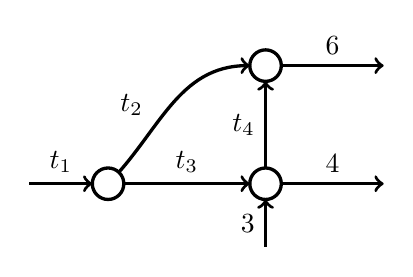
\begin{tikzpicture}
				\draw[very thick, ->] (0,0) -- (0.8,0) node[midway, above]{$t_1$};
				\draw[very thick, ->] (3.2,0) -- (4.5,0) node[midway, above]{$4$};
				\draw[very thick, ->] (1.2,0) -- (2.8,0) node[midway, above]{$t_3$};
				\draw[very thick, ->] (3,-0.8) -- (3,-0.2) node[midway, left]{$3$};
				\draw[very thick, ->] (3,0.2) -- (3,1.3) node[midway, left]{$t_4$}; 
				\draw[very thick, ->] (3.2,1.5) -- (4.5,1.5) node[midway, above]{$6$};
				\draw[very thick, ->] (1,0) to[out = 45, in = 180] (2.8,1.5);
				\draw (1.3,1) node {$t_2$};
				
				\draw[very thick, fill = white] (3,0) circle (0.2);
				\draw[very thick, fill = white] (3,1.5) circle (0.2);
				\draw[very thick, fill = white] (1,0) circle (0.2);
			\end{tikzpicture}
		\end{center}
		
		We saw in example \ref{ex:intersection} that there is an equation for each intersection. At each intersection, the cars entering the intersection must equal the cars leaving the intersection. We will further assume that no cars stay parked on these streets. Then we get the following system of linear equations.
		
		\[
			\arraycolsep=1.4pt
			\begin{array}{rcrcrcrl}
				t_1 & - & t_2 & - & t_3 & & & = 0\\
				& & t_2 & & & + & t_4 & = 6\\
				& & & & t_3 & - & t_4 & =  1
			\end{array}
		\]
		
		The corresponding augmented matrix is $\begin{bmatrix} 1 & -1 & -1 & 0 & 0 \\ 0 & 1 & 0 & 1 & 6 \\ 0 & 0 & 1 & -1 & 1\end{bmatrix}$. While this is already in row echelon form, we can further row reduce this into reduced row echelon form.
		\[
			\begin{bmatrix} 1 & -1 & -1 & 0 & 0 \\ 0 & 1 & 0 & 1 & 6 \\ 0 & 0 & 1 & -1 & 1\end{bmatrix}\qquad \xrightarrow{\text{Some row operations}} \qquad
			\begin{bmatrix} 1 & 0 & 0 & 0 & 7 \\ 0 & 1 & 0 & 1 & 6 \\ 0 & 0 & 1 & -1 & 1\end{bmatrix}
		\]
		
		From this, we can immediately see that there must be an average of 7 cars per hour entering this block from the west. This makes intuitive sense, since there are an average of 10 cars leaving this block each hour to the west and an average of 3 cars entering this block each hour from the south.

		Note that the number of cars travelling in the middle streets of the block still depend on each other once we've finished reducing the system. We cannot further eliminate these dependencies. In this case, we see tht $t_2 = 6 - t_4$ and $t_3 = 1 + t_4$. Since we can describe all of the traffic in these streets in terms of $t_4$, we will phrase our solution in terms of $t_4$. 
		
		Suppose that there are an average of $c$ cars per hour travelling down the street labelled $t_4$ so that $t_4 = c$. This gives us a complete description of our traffic flow:
		\begin{align*}
			t_1 &= 7\\
			t_2 &= 6 - c\\
			t_3 &= 1 + c\\
			t_4 &= c
		\end{align*}
		
		One possible solution to this system is given by taking $c = 4$ to give $t_4 = 2$, $t_3 = 3$, and $t_2 = 4$. Another possible solution has $c = 10$ to give $t_4 = 10$, $t_3 = 11$, and $t_2 = -5$. We could interpret this negative car flow as there being 5 more cars each heading south west on the street labelled $t_2$ than there are cars heading north east.
		
\end{example}

\begin{remark}
	In this last example, we chose not to show the steps in our row reduction to save space. This is a bad habit and you should not emulate it. When solving systems of linear equations, make sure to show all of your steps.
\end{remark}

As we have just seen, it is possible to solve a system and not completely eliminate the relationships between all of the variables. In this last example, we were able to determine that $x_1 = 7$, but $x_2, x_3,$ and $x_4$ were stll dependent on one another. In this case, we chose one of our variables to replace with a \textbf{parameter}. A parameter is a new variable which does not already have meaning within the context of the system, but with which we can completely describe the solutions of the system. In the preceeding example, choosing different values of $c$ gave us different solutions to our traffic system. It is typical to use variables $t, s, r$ for parameters, if needed. Such an expression for the solution of the linear system is called a \textbf{parametric form} for the \textbf{general solution} to the system.

Given the augmented matrix for a system in RREF, can we tell how many paramters the solution to the system has? If so, how do we choose which variables are parameters?

\begin{example}\label{ex:parameters}
	A linear system has augmented matrix $A$. After row reducing $A$, we transform it into the following reduced row echelon form.
	
	\[
		A \xrightarrow{\text{Some row operations}} 
		\begin{bmatrix} 
			1 & 0 & 3 & 4 & 0 & 6\\
			0 & 1 & 2 & 0 & 0 & -4\\
			0 & 0 & 0 & 0 & 1 & 1
		\end{bmatrix}
	\]
	
	From this, we can see that $\left\{ 
		\arraycolsep=1.4pt
		\begin{array}{rcrcrcrcrl} 
			x_1 & & & + &  3x_3 & + & 4x_4 & & & = 6\\
			      & & x_2 & + & 2x_3 & & & & & = -4\\
			      & & & & & & & & x_5 & = 1
		\end{array}
	\right.$.

	From this, we note that $x_5 = 1$ and that we can write $x_1$ and $x_2$ in terms of $x_3$ and $x_4$. Therefore, we choose $x_3$ and $x_4$ to be our parameters. Let $x_3 = s$ and $x_4 = t$. This gives us a general solution of
	\begin{align*}
		x_1 & = 6 - 3s - 4t\\
		x_2 &= -4 - 2s\\
		x_3 &= s \\
		x_4 &= t\\
		x_5 &= 1.
	\end{align*}
\end{example}

The last two examples have something in common. In example \ref{ex:traffic2}, the system had 3 variables, the final reduced row echelon augmented matrix had 2 leading 1's, and the general solution had $3-2 = 1$ parameter. In example \ref{ex:parameters}, the system had 5 variables, the final reduced row echelon augmented matrix had $3$ leading 1's, and the general solution had $5-3 = 2$ parameters. This suggests the following result.

\begin{theorem}
	If a linear system is consistent, has $n$ variables, and after row reduction the augmented matrix in row echelon form has $k$ leading $1$'s, then the general solution will have 
	\[
		\text{Number of parameters} = n - k
	\]
\end{theorem}

We can further note that in these two examples, the parameters were chosen to be variables whose corresponding columns did not have leading $1$'s. In example \ref{ex:traffic2}, we chose $t_4$ to be the parameter which corresponds to the fourth column of the RREF matrix $\begin{bmatrix} 1 & 0 & 0 & 0 & 7 \\ 0 & 1 & 0 & 1 & 6 \\ 0 & 0 & 1 & -1 & 1\end{bmatrix}$ for the system which does not contain a leading $1$. Choosing the variables whose columns do not have a leading $1$ in the REF will always work. Furthermore, this choice also requires the least amount of work when writing out the general solution.

Lastly, we need to discuss inconsistent systems. Does row reduction allow us to identify inconsistent systems? If so, how can we recognize that a linear system is inconsistent?

\begin{example}\label{ex:inconsistent}

	Suppose we have the following network of streets with traffic labelled.
	\begin{center}
			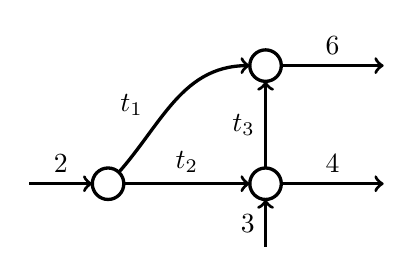
\begin{tikzpicture}
				\draw[very thick, ->] (0,0) -- (0.8,0) node[midway, above]{$2$};
				\draw[very thick, ->] (3.2,0) -- (4.5,0) node[midway, above]{$4$};
				\draw[very thick, ->] (1.2,0) -- (2.8,0) node[midway, above]{$t_2$};
				\draw[very thick, ->] (3,-0.8) -- (3,-0.2) node[midway, left]{$3$};
				\draw[very thick, ->] (3,0.2) -- (3,1.3) node[midway, left]{$t_3$}; 
				\draw[very thick, ->] (3.2,1.5) -- (4.5,1.5) node[midway, above]{$6$};
				\draw[very thick, ->] (1,0) to[out = 45, in = 180] (2.8,1.5);
				\draw (1.3,1) node {$t_1$};
				
				\draw[very thick, fill = white] (3,0) circle (0.2);
				\draw[very thick, fill = white] (3,1.5) circle (0.2);
				\draw[very thick, fill = white] (1,0) circle (0.2);
			\end{tikzpicture}
		\end{center}
		
	Intuitively, the traffic flows listed are not physically possible. There are more cars leaving this block than there are entering it. What happens when we row reduce the augmented matrix? We write out the augmented matrix for the traffic system and row reduce.
	\[
		\begin{bmatrix}
			1 & 1 & 0 & 2\\
			1 & 0 & 1 & 6\\
			0 & 1 & -1 & -1
		\end{bmatrix}
		\qquad \xrightarrow{\text{Some row operations}} 
		\begin{bmatrix}
			1 & 1 & 0 & 2\\
			0 & 1 & -1 & -4\\
			0 & 0 & 0 & 1
		\end{bmatrix}
	\]
	
	Therefore, our traffic system has the same solutions as the system 
	$\left\{
		\arraycolsep=1.4pt
		\begin{array}{rcrcrl} 
			x_1  &+ & x_2 & & & = 2\\  
			& & x_2 & - & x_3 & = -4\\
			& & & & 0 & = 1
		\end{array}
	\right.$.
	However, no choices of $x_1, x_2,$ and $x_3$ will ever make $0 = 1$ a true statement. Therefore, this system has no solutions and is inconsistent.
\end{example}

In this example, we determined that the system was inconsistent by row reducing the augmented matrix to arrive at a linear system with $0 = 1$. Fortunately, this will always happen. If a linear system is inconsistent, then its augmented matrix will row reduce into an REF matrix with a row $\begin{bmatrix} 0 & 0 & \cdots & 0 & 1\end{bmatrix}.$
